\documentclass[11pt,handout,aspectratio=169]{beamer}


%%%%%%%%% GENERAL PACKAGES
%\usepackage{xcolor}
%\usepackage{pdfpages}
%\usetheme[progressbar=frametitle]{metropolis}
%\setbeamercolor{background canvas}{bg=white}
%\usepackage{appendixnumberbeamer}
%\usepackage{booktabs}
%\usepackage[scale=2]{ccicons}
%\usepackage{pgfplots}
%\usepgfplotslibrary{dateplot}
%\usepackage{xspace}
%\newcommand{\themename}{\textbf{\textsc{metropolis}}\xspace}
%\usepackage[absolute,overlay]{textpos}

%%%%%%%%% COLOR THEME

% Define some colors:
\definecolor{DarkFern}{HTML}{407428}
\definecolor{DarkCharcoal}{HTML}{4D4944}
\definecolor{AlertColor}{RGB}{89,124,158}
\definecolor{HighLight}{RGB}{96,95,134}
\definecolor{Important}{RGB}{234,122,133}
\definecolor{Yellow}{HTML}{00539C}
\colorlet{Fern}{DarkFern!85!white}
\colorlet{Charcoal}{DarkCharcoal!85!white}
\colorlet{LightCharcoal}{Charcoal!50!white}
\colorlet{HighLight2}{AlertColor}
\colorlet{DarkRed}{red!70!black}
\colorlet{DarkBlue}{blue!70!black}
\colorlet{DarkGreen}{green!70!black}
\definecolor{RoyalBlue}{HTML}{00539C}
\definecolor{Peach}{HTML}{EEA47F}
\definecolor{ForestGreen}{HTML}{2C5F2D}
\definecolor{MossGreen}{HTML}{E8FCC9}
% Use the colors:
\setbeamercolor{title}{fg=Fern}
\setbeamercolor{frametitle}{fg=MossGreen,bg=ForestGreen}
\setbeamercolor{normal text}{fg=Charcoal!70!black}
\setbeamercolor{block title}{fg=black,bg=Fern!25!white}
\setbeamercolor{block body}{fg=black,bg=Fern!10!white}
\setbeamercolor{block title alerted}{fg=black,bg=DarkRed!25!white}
\setbeamercolor{block body alerted}{fg=black,bg=DarkRed!10!white}
\setbeamercolor{alerted text}{fg=DarkRed}
\setbeamercolor{itemize item}{fg=Charcoal}



%%%%%%%%% OTHER COMMANDS
\newcommand{\indep}{\perp\!\!\! \perp}
\newcommand{\comment}[1]{}
\newcommand{\bs}{\boldsymbol}
\newcommand{\tr}{\text{trace}}
\newcommand{\sgn}{{\rm sgn}}
\def\T{\top}
%\newcommand{\det}{\text{det}}
\newcommand{\var}{\mathrm{var}}
\newcommand{\cC}{{\cal C}}
\newcommand{\cG}{{\cal G}}
\newcommand{\cV}{{\cal V}}
\newcommand{\cE}{{\cal E}}
\newcommand{\cM}{{\cal M}}
\newcommand{\cP}{{\cal P}}
\newcommand{\cX}{{\cal X}}
\newcommand{\cY}{{\cal Y}}
\newcommand{\X}{\mathbf{X}}
\newcommand{\Y}{\mathbf{Y}}
\newcommand{\x}{\mathbf{x}}
\newcommand{\y}{\mathbf{y}}
\newcommand{\z}{\mathbf{z}}

\newcommand{\argmin}{\operatornamewithlimits{argmin}}
\newcommand{\eps}{\varepsilon}
\newcommand{\<}{\langle}
\renewcommand{\>}{\rangle}


\setbeamertemplate{itemize subitem}{\tiny\raise1.5pt\hbox{\donotcoloroutermaths$\blacktriangleright$}}
\setbeamertemplate{itemize subsubitem}{\tiny\raise1.5pt\hbox{\donotcoloroutermaths$\blacktriangleright$}}
\setbeamertemplate{enumerate item}{\insertenumlabel.}
\setbeamertemplate{enumerate subitem}{\insertenumlabel.\insertsubenumlabel}
\setbeamertemplate{enumerate subsubitem}{\insertenumlabel.\insertsubenumlabel.\insertsubsubenumlabel}
\setbeamertemplate{enumerate mini template}{\insertenumlabel}

\newcommand{\TODO}[1]{{\color{red}{[TODO: #1]}}}


\newcommand{\R}{\mathbb R}
\newcommand{\E}{\mathbb E}
\renewcommand{\P}{\mathbb P}


\DeclareMathOperator*{\cov}{cov}


\newsavebox{\zerobox}
\newenvironment{nospace}
{\par\edef\theprevdepth{\the\prevdepth}\nointerlineskip
  \setbox\zerobox=\vtop to 0pt\bgroup
  \hrule height0pt\kern\dimexpr\baselineskip-\topskip\relax
}
{\par\vss\egroup\ht\zerobox=0pt \wd\zerobox=0pt \dp\zerobox=0pt
  \box\zerobox}

\usepackage{soul}
\makeatletter
\let\HL\hl
\renewcommand\hl{%
  \let\set@color\beamerorig@set@color
  \let\reset@color\beamerorig@reset@color
  \HL}
  \makeatother


\title[STA437-Week1]{STA 437/2005: \\ Methods for Multivariate Data}
\subtitle[]{Week 10: Factor Analysis}
\author[Piotr Zwiernik]{Piotr Zwiernik}
\institute[UofT]{University of Toronto}
\date{}


%\usepackage{Sweave}

\begin{document}

\maketitle
\section{Introduction}
\begin{frame}{Low-dimensional structures in multivariate statistics}
Discussing covariance matrix estimation we mentioned some special structures that are routinely assumed in multivariate statistics. \\[4mm]

We will discuss in detail two such constraints:
\begin{itemize}
	\item $\Sigma=L+S$ where $L$ is low-rank and $S$ is sparse. 
	\item the inverse of $\Sigma^{-1}$ is sparse.\\[4mm]
\end{itemize}

In Factor Analysis: \hl{$\Sigma=WW^\top +\Psi$} with $W\in \R^{m\times r}$, $\Psi$ diagonal.\\[4mm]

We explain here how such structure can occur by discussing motivating examples.

\end{frame}




\section{Factor Analysis }

%\begin{frame}{}
%	\begin{center}
%		{\Huge \alert{Factor Analysis}}
%	\end{center}
%\end{frame}

\begin{frame}{Factor Analysis: Motivating Examples}
\begin{block}{Example: Capital Asset Pricing Model (CAPM)}
	Models stock returns based on a common factor; the \alert{market return}. For each stock:
	\[ X_i \;=\; \mu_i + w_i Z + \eps_i \]
This is one of the most basic models in finance.
\end{block}
\begin{alertblock}{Example: Human Intelligence}
	Cognitive abilities modeled by latent \alert{intelligence factor}.\\[3mm]
	This could be further generalized to account for multiple types of intelligence.
\end{alertblock}
\end{frame}

\section{Factor Analysis Model}

\begin{frame}{Factor Analysis Model}
The model assumes the following stochastic representation of $X=(X_1,\ldots,X_m)$:
\[ X = \mu + WZ + \eps, \qquad Z\sim N_r(0, I_r),\quad \eps \sim N_m(0, \Psi), \quad Z\indep \eps,\]
where $\Psi$ is a diagonal covariance matrix.
        \begin{block}{The latent factors $Z$}
        	As the two examples suggest, often in this context $Z$ has a specific interpretation.
        \end{block}
      \bigskip     
In PPCA we have the same representation with $\Psi=\sigma^2 I_m$ (isotropic noise).\\[4mm]

In FA more emphasis on interpreting the latent factors.
\end{frame}

\begin{frame}{Parametrization and identifiability}
	$X=\mu+WZ+\eps$ is Gaussian with the induced covariance structure: \[ \Sigma \;=\; \textcolor{blue}{WW^T} + \alert{\Psi}. \]
%	Note that this model equals to Probabilistic PCA if $\Psi=\sigma^2I_m$.\\[4mm]
%	Unlike in PPCA there is no analytic formula for the MLE. \\[4mm]
\begin{alertblock}{Lack of identifiability}
	As for PPCA, $W$ is not uniquely identified.
	\begin{itemize}
		\item Replacing $W$ with $WU$ for $U\in O(m)$ does not change the distribution.
		\item This has important consequences for model intepretability.
	\end{itemize}
\end{alertblock}
\end{frame}

\begin{frame}{Dealing with non-uniqueness of $W$}
\textbf{Approach 1: } Constraint $W$ so that $W^T\Psi^{-1}W$ diagonal.
    \begin{itemize}
        \item Multiply $X=\mu+WZ+\eps$ by $\Psi^{-1/2}$ to get $\tilde X=\tilde \mu+\tilde WZ+\tilde \eps$ with $\tilde\eps\sim N(0,I_m)$.
        \item We have $W^T\Psi^{-1}W=\tilde W^\top \tilde W$ so this corresponds to orthogonality of the columns of $\tilde W^\top$.
    \end{itemize}
    \bigskip
    
    \textbf{Approach 2: } Apply \alert{varimax rotation} for interpretability.
    \begin{itemize}
    	\item Consider any $\widehat W\in \R^{m\times r}$. We find $U$ such that $\widehat WU$ more interpretable. 
    	\item Define $M\in \R^{m\times r}$ by $M_{ij}=\frac{(WU)_{ij}^2}{\sum_{k=1}^r (WU)_{ij}^2}$ then find the appropriate $U$ \textcolor{blue}{maximizing}: 
    	$$\|M-\tfrac1m \bs 1_m\bs 1_m^\top M\|^2_F.$$
    	\item This results with solutions such that each column of $M$ has a bunch of big entries and the remaining ones are negligible.
    \end{itemize}
\end{frame}

\begin{frame}{Fitting the factor analysis model}
Data: $\x_1,\ldots,\x_n$ from the model $X=\textcolor{blue}{\mu}+\textcolor{blue}{W}Z+\eps$, $\eps\sim N(0,\textcolor{blue}{\Psi})$.\\[3mm]
	The most canonical way to estimate the parameters is via the maximum likelihood. \\[3mm]
	The MLE is not given in a closed form. 
	\begin{itemize}
		\item We could use the EM algorithm.
	\end{itemize}
	\begin{block}{Alternatively use the fact that MLE has closed form if $\Psi=\sigma^2 I_m$.}
	Suppose $\Psi$ is known.\\[3mm] Denote $\tilde X=\Psi^{-1/2}X$, $\tilde \mu=\Psi^{-1/2}\mu$, $\tilde W=\Psi^{-1/2}W$ and $\tilde\eps =\Psi^{-1/2}\eps\sim N(0,I_m)$
	$$\tilde X=\tilde \mu+\tilde W Z+\tilde \eps. \quad(\mbox{PPCA with $\sigma^2=1$})$$
	\end{block}
\end{frame}

\begin{frame}{}
\begin{block}{}
	Define $\tilde S_n=\Psi^{-1/2}S_n\Psi^{-1/2}$ with spectral decomposition $\tilde S_n=U\tilde\Lambda U^\top$. The MLE:
	$$
	\widehat W\;=\;U_r \Theta R,
	$$
	where:
	\begin{itemize}
		\item $R$ is \emph{any} orthogonal matrix, $U_r$ first $r$ columns of $U$,
		\item $\Theta$ is a diagonal matrix with $i$-th entry equal to $\sqrt{\max\{0,\tilde \lambda_i-1\}}$.
	\end{itemize}
\end{block}
We can now apply this iteratively, where the update on $\Psi$ 
	\end{frame}

\begin{frame}{Choosing the Number of Factors}
Determining the number of latent factors \( r \) is critical in factor analysis.\\[4mm]  
Overestimating \( r \) leads to overfitting, underestimating \( r \) leads to loss of structure.\\[4mm]
There are several common method. We focus on Horn's Parallel Analysis (PA).
%Common methods:
%    \begin{itemize}
%      \item Scree plots (eigenvalue-based heuristics)
%      \item Information-theoretic criteria (AIC, BIC)
%      \item Velicer's MAP test
%      \item \textbf{Horn's Parallel Analysis (PA)}
%    \end{itemize}
%    \medskip
%    
\begin{alertblock}{Key ideas of Horn's Parallel Analysis}
	If no latent signal, the sample \textbf{correlation} matrix should resemble the identity matrix.\\[4mm]
	Depending on $(n,m)$ the actual eigenvalues can still be far from 1.
\end{alertblock}

 PA compares eigenvalues of observed data with those obtained from Monte Carlo simulations of purely random noise.\end{frame}



\begin{frame}{Horn's Parallel Analysis}
Based on the observed data $\bs X\in \R^{n\times m}$:
  \begin{enumerate}
    \item Compute eigenvalues \( \lambda_1 \geq \lambda_2 \geq \dots \geq \lambda_m \) of sample correlation matrix \( R_n \), where
    \begin{equation}
      R_n = D^{-1/2} S_n D^{-1/2}.
    \end{equation}
    \item Generate \( B \) simulated datasets \(\bs X^{(b)} \in \mathbb{R}^{n \times m} \) from \( {N}_m(\bs 0,I_m) \).
    \item Compute sample correlation matrices \( R_n^{(b)} \) for each simulated dataset.
    \item Compute average null eigenvalues:
    \begin{equation}
      \lambda_j^{\text{random}} = \frac{1}{B} \sum_{b=1}^{B} \lambda_j^{(b)}, \quad j = 1, \dots, m.
    \end{equation}
    \item Retain factors where
    \begin{equation}
      \lambda_j > \lambda_j^{\text{random}}.
    \end{equation}
  \end{enumerate}
\end{frame}


\begin{frame}{Application: Factor Analysis on Personality Traits Data}
We analyze real survey data from the \texttt{bfi} dataset in the \texttt{psych} R package.\\[4mm]
The dataset consists of 2,800 responses to 25 personality-related questions.\\[4mm]
These questions measure the Big Five Personality Traits:
    \begin{itemize}
      \item Neuroticism (N)
      \item Extraversion (E)
      \item Conscientiousness (C)
      \item Agreeableness (A)
      \item Openness (O)
    \end{itemize}
Responses are on the 1-6 scale indicating agreement strength.\\[4mm]

We discard demographic variables (gender, age, education).
\end{frame}

\begin{frame}{Factor Analysis Results}
\alert{PA} suggests retaining \textbf{five} factors, matching the Big Five personality traits (nice!).\\[4mm]
Factor loadings after \alert{varimax rotation} confirm that the extracted factors correspond to the expected latent traits.
\begin{center}
    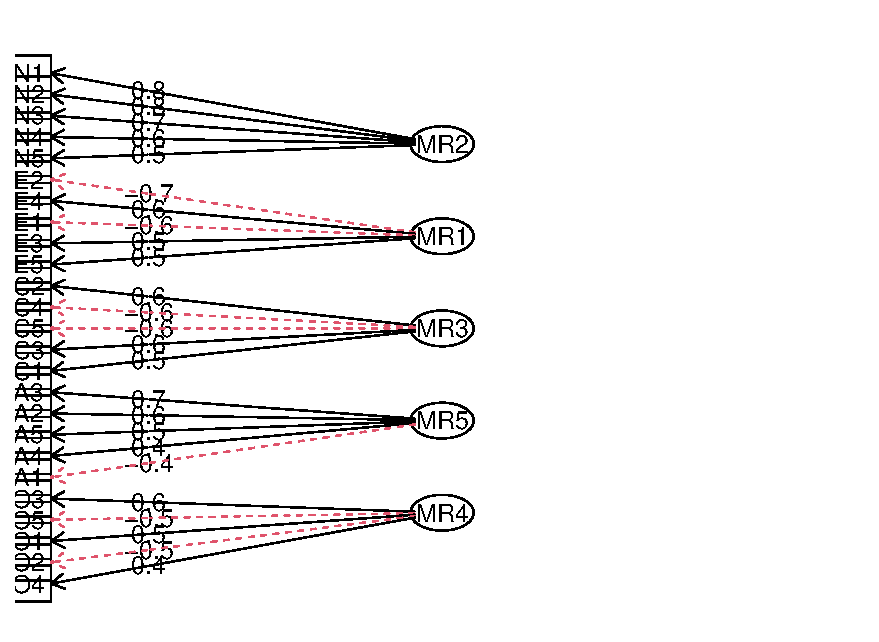
\includegraphics[width=0.3\linewidth]{pics/FA.pdf}	
\end{center}
\end{frame}

\begin{frame}{Summary}
	Factor Analysis is a popular method in multivariate statistics. \\[4mm]
	It is similar to PPCA and it has clear motivating examples. \\[4mm]
	The lack of identifiability creates a chalange in the interetation of factor loadings.\\[4mm]
	Choosing the number of factors (if there is no clear insight) may be also hard. 
	\begin{itemize}
		\item Horn's Parallel Analysis is a simple solution that tends to perform well in practice.\\[4mm]
	\end{itemize}
	The resulting form of the covariance matrix $\Sigma=WW^\top +\Psi$ can be exploited and generalized in many creative ways. 
\end{frame}

%\section{Independent Component Analysis (ICA)}
%
%\begin{frame}{ICA: Motivating Examples}
%    \textbf{Example: Cocktail Party Problem}
%    \begin{itemize}
%        \item Separate mixed audio signals into independent sources.
%        \item Modeled as: \[ X = WZ \]
%    \end{itemize}
%    \textbf{Example: EEG/MEG Analysis}
%    \begin{itemize}
%        \item Extract independent brain signals from mixed recordings.
%    \end{itemize}
%\end{frame}
%
%
%
%\begin{frame}{ICA Model}
%    \begin{itemize}
%        \item Observed signal: \[ X = WZ \]
%        \item Assumes $Z$ has independent non-Gaussian components.
%        \item Identifiability result: Unique up to permutation and scaling.
%    \end{itemize}
%\end{frame}
%
%\begin{frame}{ICA: Non-Gaussianity Principle}
%    \begin{itemize}
%        \item Gaussian components remain Gaussian under rotation.
%        \item Non-Gaussian components allow identification.
%        \item Theorem (Comon): If at most one component is Gaussian, $W$ is identifiable up to permutation and scaling.
%    \end{itemize}
%\end{frame}
%
%\section{Estimation Methods}
%
%\begin{frame}{Factor Analysis Estimation: MLE}
%    \begin{itemize}
%        \item Log-likelihood maximization.
%        \item EM algorithm: iteratively estimates $W$ and $\Psi$.
%        \item J\"oreskog's method: Spectral decomposition approach.
%    \end{itemize}
%\end{frame}
%
%\begin{frame}{ICA Estimation: Method of Moments}
%    \begin{itemize}
%        \item Uses higher-order statistics (kurtosis, skewness).
%        \item JADE algorithm: Estimates mixing matrix via cumulants.
%        \item Contrast functions: Measures independence.
%    \end{itemize}
%\end{frame}


\end{document}

